\documentclass[tikz,border=5pt]{standalone}
\usepackage[T1]{fontenc}
\usepackage{lmodern,amsmath,amssymb}
\usetikzlibrary{arrows.meta,calc,positioning,fit,backgrounds,shapes.geometric,matrix,decorations.pathreplacing,patterns}
\definecolor{ink}{gray}{0.08}
\definecolor{wash}{gray}{0.965}
\definecolor{soft}{gray}{0.45}
\tikzset{box/.style={draw=ink,line width=.65pt,fill=white,align=center,inner sep=4pt,outer sep=0pt,font=\small},flow/.style={draw=ink,line width=.65pt,-{Latex[length=1.8mm,width=1.3mm]},rounded corners=2pt},annotation/.style={font=\scriptsize,text=soft,align=center},groupbox/.style={draw=soft,dashed,line width=.45pt,fill=wash}}
\begin{document}
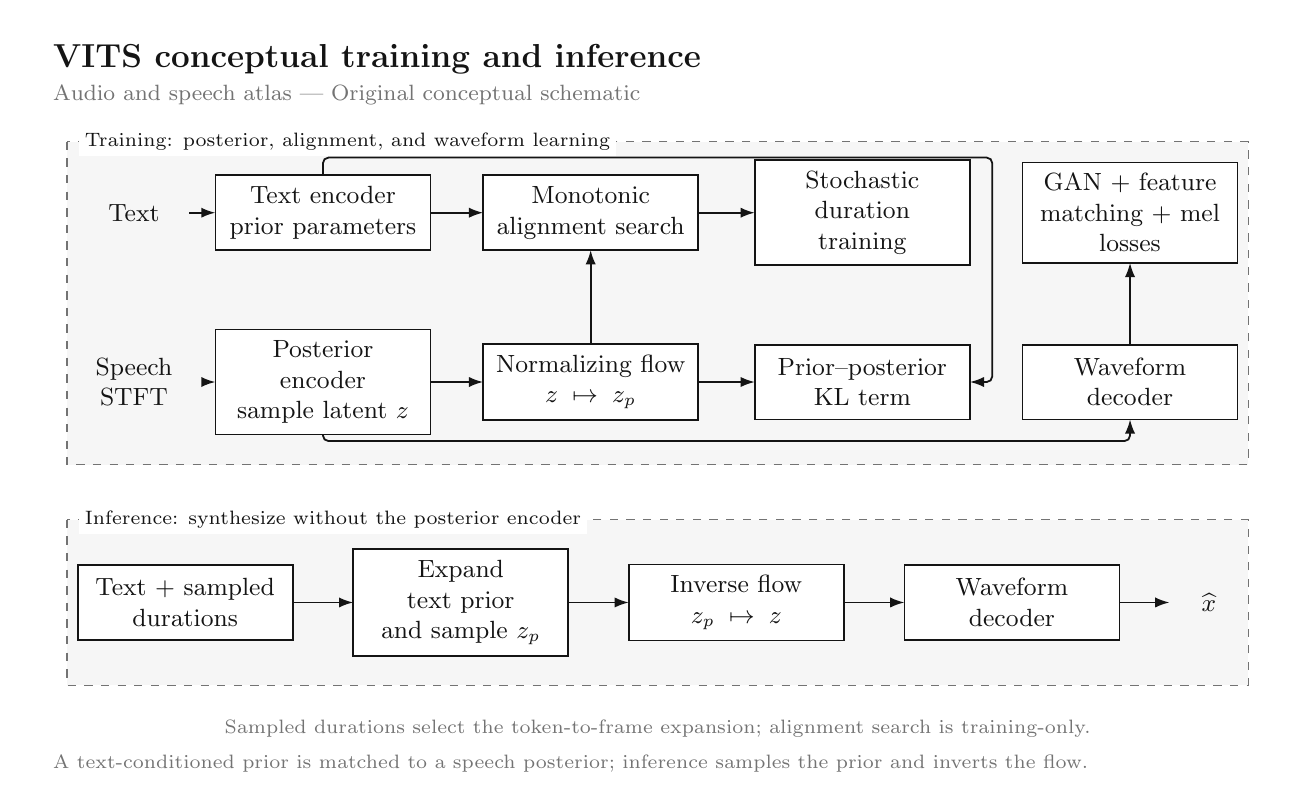
\begin{tikzpicture}[x=1cm,y=-1cm,font=\rmfamily,text=ink]

\path[use as bounding box] (0,0) rectangle (16,9.6);
\node[anchor=west,font=\large\bfseries] at (.2,.4) {VITS conceptual training and inference};
\node[anchor=west,font=\footnotesize,text=soft] at (.2,.85) {Audio and speech atlas | Original conceptual schematic};
\begin{pgfonlayer}{background}
\draw[groupbox] (0.5,1.45) rectangle (15.5,5.55);
\node[anchor=west,font=\scriptsize,fill=white,inner sep=2pt] at (0.65,1.45) {Training: posterior, alignment, and waveform learning};
\draw[groupbox] (0.5,6.25) rectangle (15.5,8.35);
\node[anchor=west,font=\scriptsize,fill=white,inner sep=2pt] at (0.65,6.25) {Inference: synthesize without the posterior encoder};
\end{pgfonlayer}
\node[align=center,inner sep=0pt,outer sep=0pt,font=\small,minimum width=1.4cm,minimum height=0.75cm,text width=1.15cm] (textT) at (1.35,2.35) {Text};
\node[box,minimum width=2.7cm,minimum height=0.95cm,text width=2.45cm] (prior) at (3.75,2.35) {Text encoder\\prior parameters};
\node[box,minimum width=2.7cm,minimum height=0.95cm,text width=2.45cm] (mas) at (7.15,2.35) {Monotonic\\alignment search};
\node[box,minimum width=2.7cm,minimum height=0.95cm,text width=2.45cm] (dur) at (10.6,2.35) {Stochastic duration\\training};
\node[box,minimum width=2.7cm,minimum height=0.95cm,text width=2.45cm] (gan) at (14.0,2.35) {GAN + feature\\matching + mel\\losses};
\node[align=center,inner sep=0pt,outer sep=0pt,font=\small,minimum width=1.9cm,minimum height=0.95cm,text width=1.65cm] (speech) at (1.35,4.5) {Speech\\STFT};
\node[box,minimum width=2.7cm,minimum height=0.95cm,text width=2.45cm] (posterior) at (3.75,4.5) {Posterior encoder\\sample latent $z$};
\node[box,minimum width=2.7cm,minimum height=0.95cm,text width=2.45cm] (flow) at (7.15,4.5) {Normalizing flow\\$z\mapsto z_p$};
\node[box,minimum width=2.7cm,minimum height=0.95cm,text width=2.45cm] (kl) at (10.6,4.5) {Prior--posterior\\KL term};
\node[box,minimum width=2.7cm,minimum height=0.95cm,text width=2.45cm] (decT) at (14.0,4.5) {Waveform decoder};
\node[box,minimum width=2.7cm,minimum height=0.95cm,text width=2.45cm] (textI) at (2.0,7.3) {Text + sampled\\durations};
\node[box,minimum width=2.7cm,minimum height=0.95cm,text width=2.45cm] (sample) at (5.5,7.3) {Expand text prior\\and sample $z_p$};
\node[box,minimum width=2.7cm,minimum height=0.95cm,text width=2.45cm] (inverse) at (9.0,7.3) {Inverse flow\\$z_p\mapsto z$};
\node[box,minimum width=2.7cm,minimum height=0.95cm,text width=2.45cm] (decI) at (12.5,7.3) {Waveform decoder};
\node[align=center,inner sep=0pt,outer sep=0pt,font=\small,minimum width=1.0cm,minimum height=0.95cm,text width=0.75cm] (audio) at (15.0,7.3) {$\widehat{x}$};
\begin{pgfonlayer}{background}
\draw[flow] (textT.east) -- (prior.west);
\draw[flow] (prior.east) -- (mas.west);
\draw[flow] (mas.east) -- (dur.west);
\draw[flow] (speech.east) -- (posterior.west);
\draw[flow] (posterior.east) -- (flow.west);
\draw[flow] (flow.east) -- (kl.west);
\draw[flow] (flow.north) -- (mas.south);
\draw[flow] (decT.north) -- (gan.south);
\draw[flow] (prior.north) -- (3.75,1.65) -- (12.25,1.65) -- (12.25,4.5) -- (kl.east);
\draw[flow] (posterior.south) -- (3.75,5.25) -- (14.0,5.25) -- (decT.south);
\draw[flow] (textI.east) -- (sample.west);
\draw[flow] (sample.east) -- (inverse.west);
\draw[flow] (inverse.east) -- (decI.west);
\draw[flow] (decI.east) -- (audio.west);
\end{pgfonlayer}
\node[align=center,anchor=center,font=\scriptsize,text=soft,text width=14cm] at (8,8.9) {Sampled durations select the token-to-frame expansion; alignment search is training-only.};
\node[anchor=west,align=left,font=\scriptsize,text=soft,text width=15.6cm] at (.2,9.35) {A text-conditioned prior is matched to a speech posterior; inference samples the prior and inverts the flow.};
\end{tikzpicture}
\end{document}
